\documentclass{article}
\usepackage{graphicx}
\graphicspath{ { } }
\begin{document}
\title{CS 124 Programming Assignment 2}
\author{30943147}
\maketitle
\section*{Caching for the Naive Algorithm}
When multiplying two matrices $A*B=C$ using the naive matrix multiplication method, the elements of C are given as follows
$$C[i][j] = \sum\limits_k A[i][k]*B[k][j]$$
This is naturally implemented with 3 nested for loops iterating over $i$, $j$, and $k$. There are $3!=6$ possible permutations of their order. I tested all of them experimentally to determine which was best. Runtime measurements were taken by running the naive algorithm on $n \times n$ matrices with randomly generated entries for $n=1200$. 
\begin{center}
\begin{tabular}{ |c|c| } 
 \hline
 ordering & runtime\\ 
\hline
 i, j, k &  5.81s \\ 
\hline
 i, k, j & 1.73s \\ 
\hline
j, i, k & 5.54s \\
\hline
j, k, i & 25.30s\\
\hline
k, i, j & 2.05s \\
\hline
k, j, i & 24.67s\\
 \hline
\end{tabular}
\end{center}
The ordering i, k, j produces the best results. The caching behaviour of that ordering can be further optimized by saving the intermediate value of each $A[i][k]$ before we iterate over $j$. This allows the innermost loop, with iterates over $j$, to only access a single row of matrix $B$, in order, via calls to access $B[k][j]$. Since the matrices are stored in row-major order, this is very cache friendly. Saving the intermediate value of $A[i][k]$ prevents the cache from thrashing as it must repeatedly load up $A[i]$ to recalculate $A[i][k]$, which is wasted work since $A[i][k]$ isn't changing during the innermost loop over $j$. This improves runtime of the naive algorithm by an additional factor of 2-3, which drastically affects my results for $n_0$ (discussed more in the experimental results section).  

\section*{Strassen's Algorithm Implementation}
Wikipedia defines Strassen's algorithm as follows:\\
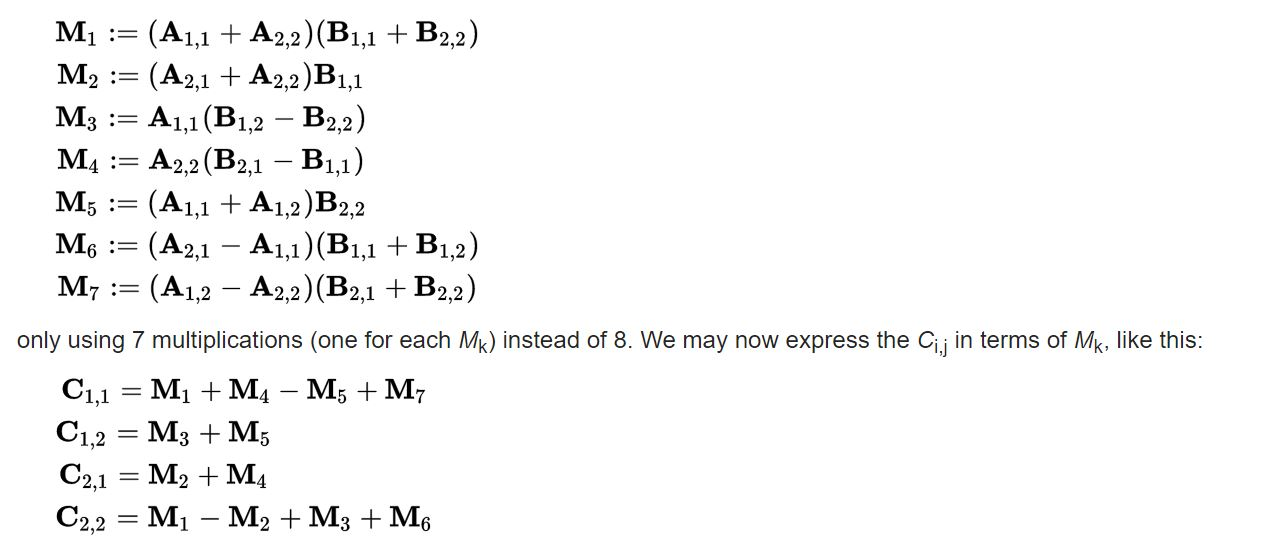
\includegraphics [scale = 0.4] {strassen} \\
I will use their variable naming scheme, both in my writeup and in my code. $A_{1,1}$ refers to the top right quadrant of $A$, and so on. 

One way to implement this code would be to define every matrix named in the above description, then carry out every computation explicitely. My algorithm sacrifices that readibility in favor of having to define fewer variables (and therefore allocate more space) and copy data from one matrix to another fewer times. 


\section*{Experimental Results for $n_0$}
\subsection*{Testing Correctness}
I used the unused first parameter as input for $n_0$ to determine what the experimental value for the optimal $n-0$ is. The program will default to whatever I determine that value to be if 0 is input for the first parameter (as the problem set description said it would be for grading). I wrote a bash script called check to help me test correctness, that would run the program first on an inputted $n_0 < n$, then on $n_0 > n$, and use the shell diff command to check that their respective outputs are identical. When $n_0 < n$, Strassen's algorithm will be used at least once. When $n_0 > n$, only the traditional matrix multiplication algorithm will be used. Therefore, this process checks my implementation of Strassen's algorithm against the traditional matrix multiplication algorithm. 
\subsection*{Runtime for Different $n_0$}
I wrote another bash script called testn0 to experiment efficiently with timing the runtime of different values of $n$ and $n_0$. I was curious if the value of the optimal crossover point might vary with $n$ as well as with $n_0$. It seemed natural to test powers of 2 for $n_0$, and I experimented with several different values of $n$. I averaged over 5 trials to reduce statistical variation. The first entry in the table, with $n_0 > n$, represents using the traditional multiplication algorithm.
\begin{center}
\begin{tabular} { |c|c|c| }
\hline
$n$ & $n_0$ & runtime \\
\hline\hline
1000 & $>1000$ & 0.82s \\
\hline\hline
1000 & 64 & 1.38s \\
\hline
1000 & 128 & 0.83s \\
\hline
1000 & 256 & 0.82s \\
\hline
1000 & 512 & 0.67s \\ 
\hline
\end{tabular}
\end{center}
$ n_0 \approx 512$ looks promising. We experiment with a few more values of $n$. 
\begin{center}
\begin{tabular} { |c|c|c| }
\hline
$n$ & $n_0$ & runtime \\
\hline\hline
2000 & $>2000$ & 4.43s \\
\hline\hline
2000 & 64 & 5.36s \\
\hline
2000 & 128 & 3.47s \\
\hline
2000 & 256 & 2.76s\\
\hline
2000 & 512 & 2.77s \\ 
\hline
2000 & 1024 & 3.83s\\
\hline
\end{tabular}
\end{center}

\begin{center}
\begin{tabular} { |c|c|c| }
\hline
$n$ & $n_0$ & runtime \\
\hline\hline
1500 & $>1500$ & 2.11s \\
\hline\hline
1500 & 64 & 2.72 s \\
\hline
1500 & 128 & 2.10s \\
\hline
1500 & 256 & 1.68s\\
\hline
1500 & 512 & 1.45s \\ 
\hline
1500 & 1024 & 1.78s\\
\hline
\end{tabular}
\end{center}

\begin{center}
\begin{tabular} { |c|c|c| }
\hline
$n$ & $n_0$ & runtime \\
\hline\hline
2500 & $>2500$ & 8.80 s \\
\hline\hline
2500 & 64 &  13.59 s \\
\hline
2500 & 128 & 8.60 s \\
\hline
2500 & 256 &  6.85 s\\
\hline
2500 & 512 & 6.33 s \\ 
\hline
2500 & 1024 & 5.40 s\\
\hline
\end{tabular}
\end{center}

$n_0 = 512$ seems to be producing the best result, ie to use Strassen's algorithm for $n \geq 512$ and not use Strassen's algorithm for $n < 512$. This was much higher than the values for $n_0$ that my classmates seemed to be getting. I am convinced that the majority of the difference comes not from slowness in my Strassen's algorithm, but from the optimizations I did for my naive multiplication algorithm. Not only did I rearrange the matrix order as suggested, but I also saved some intermediate values (discussed above). Saving intermediate values speeds up the naive multiplication algorithm by an additional factor of 2-3 in my tests, which has the consequence of pushing $n_0$ much higher than it would be if I disabled that. In fact, when I commented out that cacheing optimization, I got values of $n_0$ as low as 64. 

This table gives results for $n_0$ with the correct $i$, $j$, $k$ ordering but without the additional caching optimization on the naive algorithm.
\begin{center}
\begin{tabular} { |c|c|c| }
\hline
$n$ & $n_0$ & runtime \\
\hline\hline
1024 & $>1024$ &  1.9 s\\
\hline\hline
1024 & 32 & 1.8 s \\
\hline
1024 & 64  & 1.4 s \\
\hline
1024 & 128 & 1.4 s\\
\hline
1024 & 256 & 1.5 s\\
\hline
1024 & 512 & 1.5 s \\ 
\hline
1024 & 1024 & 1.6 s\\
\hline
\end{tabular}
\end{center}

\end{document}
